\begin{enumerate}[label=\thesection.\arabic*.,ref=\thesection.\theenumi]
\numberwithin{equation}{enumi}

\begin{abstract}
This document contains the solution to a Lines and planes problem.
\end{abstract}
Download all python codes from 
%
\begin{lstlisting}
https://github.com/sahilsin/AI_ML/Assignment 1/codes
\end{lstlisting}

\section{Problem}
Find the intersection of the following lines.
\begin{align*}
A)
    \myvec{1  &  1}\vec{x}=14
\\
    \myvec{1 & -1}\vec{x}=4
\\ \\
B)
    \myvec{1  &  -1}\vec{x}=3
\\
    \myvec{\cfrac{1}{3} & \cfrac{1}{2}}\vec{x}=6
\\ \\
C)
    \myvec{3  &  -1}\vec{x}=3
\\
    \myvec{9 & -3}\vec{x}=9
\\ \\
D)
    \myvec{0.2  &  0.3}\vec{x}=1.3
\\
    \myvec{0.4 & 0.5}\vec{x}=2.3
\\ \\
E)
    \myvec{\sqrt{2}  &  \sqrt{3}}\vec{x}=0
\\
    \myvec{\sqrt{3} & \sqrt{8}}\vec{x}=0
\\ \\
F)
    \myvec{\cfrac{3}{2}  &  \cfrac{-5}{3}}\vec{x}=-2
\\
    \myvec{\cfrac{1}{3} & \cfrac{1}{2}}\vec{x}=\cfrac{13}{6}
\end{align*}


\section{Solution}

\item The \textbf{Approach} is :

\begin{flushleft}
    For finding the intersection of these lines we will take these equations in augmented matrix form and convert left part of matrix into identity matrix and the part left on right or the last column of the matrix will give the intersection of value ,after converting left part into a identity matrix.\\
\end{flushleft}

A)
We converted these line vectors in augmented matrix form:\\ 

\begin{align*}
    \myvec{1 & 1 & 14\\1 & -1 & 4}\\
\end{align*} 

Now We will apply Row elementary operation to convert left part of matrix to identity matrix.\\

\begin{align*}
    \xleftrightarrow[]{R_{2}=R_{2}-R_{1}} \myvec{1 & 1 & 14\\1 & -2 & -10}
\\
    \xleftrightarrow[]{R_{2}=\frac{R_{2}}{-2}} \myvec{1 & 1 & 14\\0 & 1 & 5}
\\
    \xleftrightarrow[]{R_{1}=R_{1}-R_{2}} \myvec{1 & 0 & 9\\0 & 1 & 5}
\end{align*}

As left part is converted into a identity matrix the intersection vector is \myvec{9 \\ 5}\\
    
\renewcommand{\thefigure}{\theenumi.\arabic{figure}}
\begin{figure}[!ht]
    \centering
    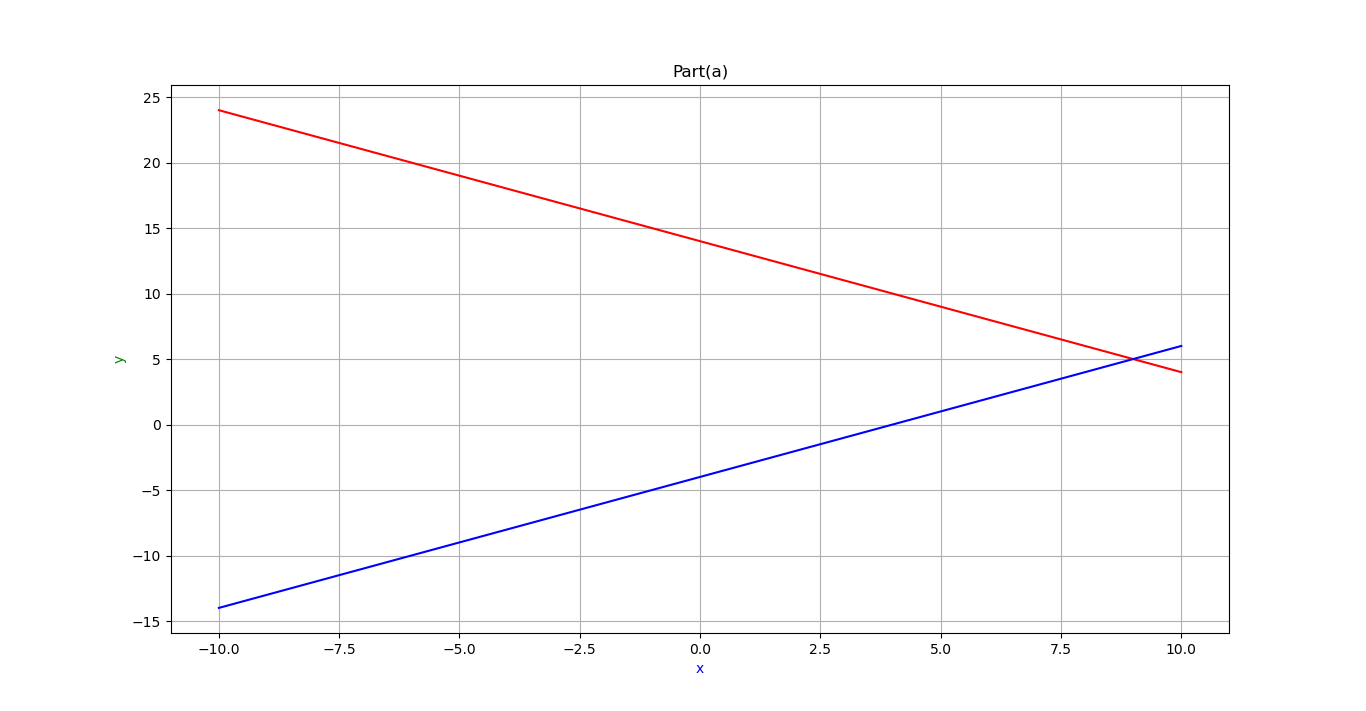
\includegraphics[width=\columnwidth]{./figures/A1_parta}
\caption{part(a)}
\label{fig: part(a)}
\end{figure}

B)
We converted these line vectors in augmented matrix form:\\ 

\begin{align*}
    \myvec{1 & -1 & 3 \\ \cfrac{1}{3} & \cfrac{1}{2} & 6}
\\ 
    \xleftrightarrow[]{R_{2}=6\times R_{2}}  \myvec{1 & -1 & 3\\2 & 3 & 36}
\\ 
    \xleftrightarrow[]{R_{2}=R_{2}-2\times R_{1}} \myvec{1 & -1 & 3\\0 & 5 & 30}
\\ 
    \xleftrightarrow[]{R_{2}=\frac{R_{2}}{5}} \myvec{1 & -1 & 3\\0 & 1 & 6}
\\ 
    \xleftrightarrow[]{R_{1}=R_{1}+R_{2}} \myvec{1 & 0 & 9\\0 & 1 & 6}
\end{align*}

As left part is converted into a identity matrix the intersection vector is \myvec{9 \\ 6}\\

\renewcommand{\thefigure}{\theenumi.\arabic{figure}}
\begin{figure}[!ht]
    \centering
    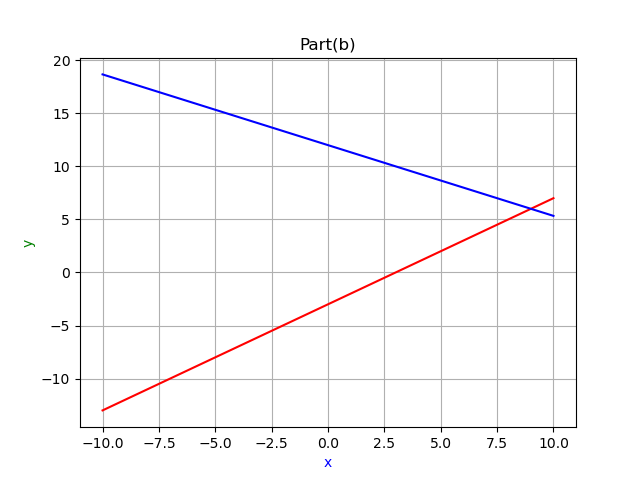
\includegraphics[width=\columnwidth]{./figures/A1_partb}
\caption{part(b)}
\label{fig: part(b)}
\end{figure}

C)
We converted these line vectors in augmented matrix form:\\ 

\begin{align*}
    \myvec{3 & -1 & 3\\9 & -3 & 9}
\\
    \xleftrightarrow[]{R_{2}=\frac{R_{2}}{3}} \myvec{1 & -1 & 3\\1 & -1 & 3}
\end{align*}

As $R_{1}=R_{2}$ , left part can never be converted into a identity matrix , and we can see now both row are same that means both lines are same they intersect at infinitely many points.\\

\renewcommand{\thefigure}{\theenumi.\arabic{figure}}
\begin{figure}[!ht]
    \centering
    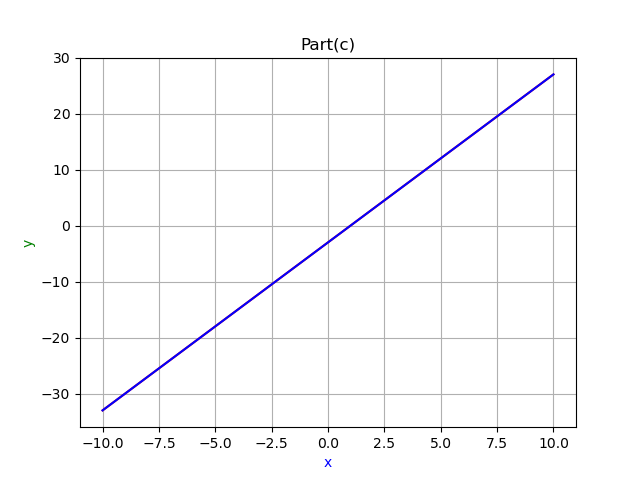
\includegraphics[width=\columnwidth]{./figures/A1_partc}
\caption{part(c)}
\label{fig: part(c)}
\end{figure}

D)
We converted these line vectors in augmented matrix form:\\ 

\begin{align*}
    \myvec{0.2 & 0.3 & 1.3\\0.4 & 0.5 & 2.3}
\\
    \xleftrightarrow[]{R_{2}=R_{2}-2\times R_{1}} \myvec{0.2 & 0.3 & 1.3\\0 & -0.1 & -0.3}
\\
    \xleftrightarrow[]{R_{2}=\frac{R_{2}}{-0.1}} \myvec{0.2 & 0.3 & 1.3\\0 & 1 & 3}
\\
    \xleftrightarrow[]{R_{1}=R_{1}-0.3 \times R_{2}} \myvec{0.2 & 0 & 0.4\\0 & 1 & 3}
\\
    \xleftrightarrow[]{R_{1}=\frac{R_{1}}{0.2}} \myvec{1 & 0 & 2\\0 & 1 & 3}
\end{align*}

As left part is converted into a identity matrix the intersection vector is \myvec{2 \\ 3}\\

\renewcommand{\thefigure}{\theenumi.\arabic{figure}}
\begin{figure}[!ht]
    \centering
    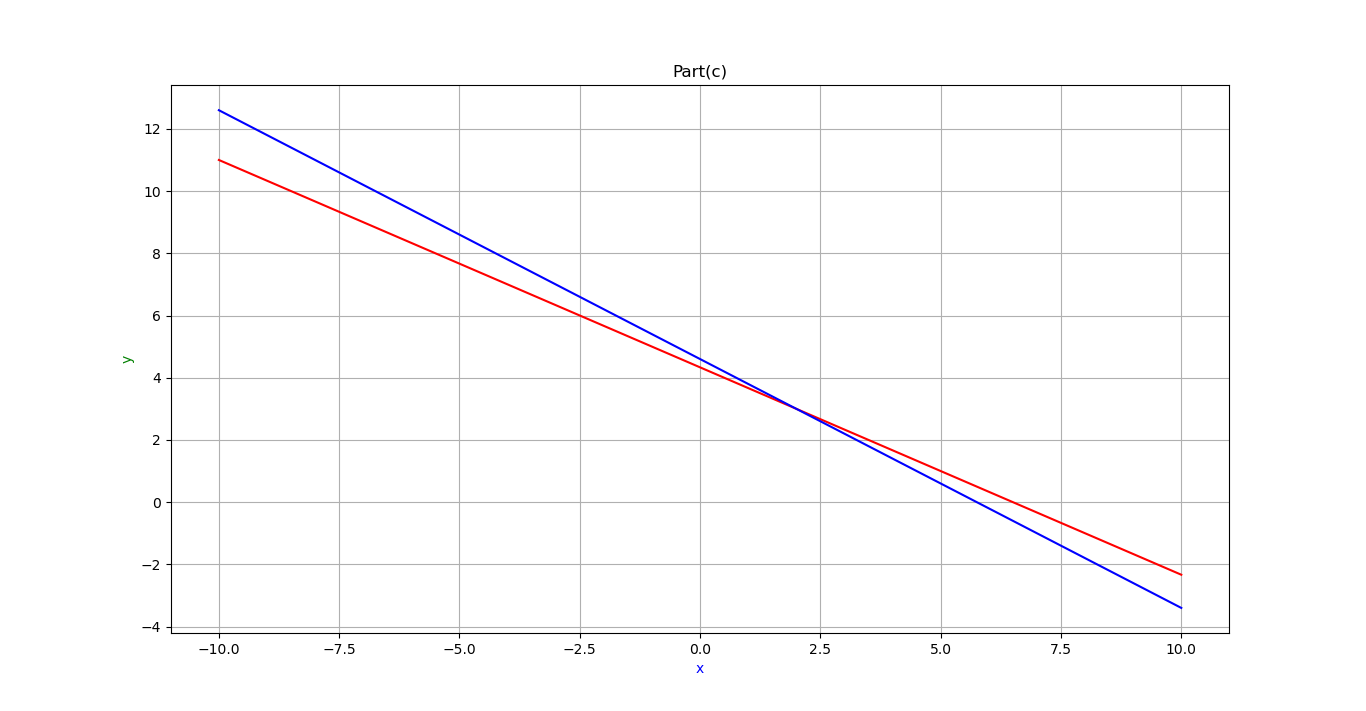
\includegraphics[width=\columnwidth]{./figures/A1_partd}
\caption{part(d)}
\label{fig: part(d)}
\end{figure}

E)
We converted these line vectors in augmented matrix form:\\ 

\begin{align*}
    \myvec{\sqrt{2} & \sqrt{3} & 0\\\sqrt{3} & \sqrt{8} & 0}
\\
    \xleftrightarrow[]{R_{2}=R_{2}-\frac{\sqrt{3}}{\sqrt{2}}\times R_{1}} \myvec{\sqrt{2} & \sqrt{3} & 0\\0 & \cfrac{1}{\sqrt{2}} & 0}
\end{align*}

As we see whatever operation we are applying last column of our augmented matrix remains zero.So the lines are homogeneous lines and they always pass through  origin , the intersection vector is \myvec{0 \\ 0}\\

\renewcommand{\thefigure}{\theenumi.\arabic{figure}}
\begin{figure}[!ht]
    \centering
    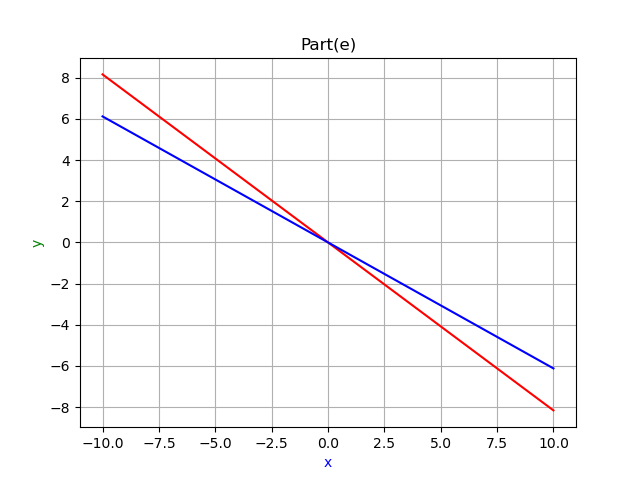
\includegraphics[width=\columnwidth]{./figures/A1_parte}
\caption{part(e)}
\label{fig: part(e)}
\end{figure}

F)
We converted these line vectors in augmented matrix form:\\ 

\begin{align*}
    \myvec{\cfrac{3}{2} & \cfrac{-5}{3} & -2\\\cfrac{1}{3} & \cfrac{1}{2} & \cfrac{13}{6}}
\\
    \xleftrightarrow[]{R_{1}=6\times R_{1}}
    \xleftrightarrow[]{R_{2}=6\times R_{2}} \myvec{9 & -10 & -12\\2 & 3 & 13}
\\
    \xleftrightarrow[]{R_{1}=R_{1}-4\times R_{2}} \myvec{1 & -22 & -64\\2 & 3 & 13}
\\
    \xleftrightarrow[]{R_{2}=R_{2}-2\times R_{1}}  \myvec{1 & -22 & -64\\0 & 47 & 141}
\\
    \xleftrightarrow[]{R_{2}=\frac{R_{2}}{47}}  \myvec{1 & -22 & -64\\0 & 1 & 3}
\\
    \xleftrightarrow[]{R_{1}=R_{1}+22\times R_{2}} \myvec{1 & 0 & 2\\0 & 1 & 3}
\end{align*}

As left part is converted into a identity matrix the intersection vector is \myvec{2 \\ 3}\\

\renewcommand{\thefigure}{\theenumi.\arabic{figure}}
\begin{figure}[!ht]
    \centering
    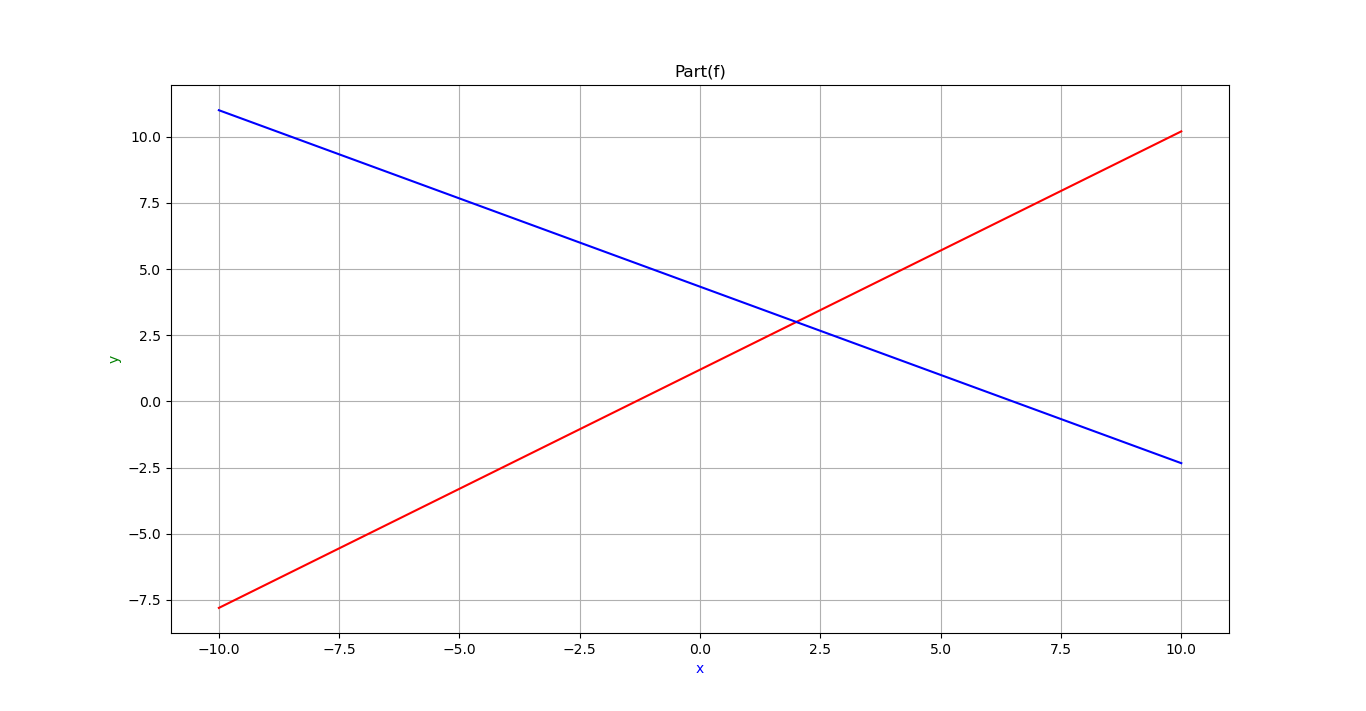
\includegraphics[width=\columnwidth]{./figures/A1_partf}
\caption{part(f)}
\label{fig: part(f)}
\end{figure}

\end{enumerate}


